\chapter*{2023年\textsf{HDU}「大学物理1」期中试题解答}

\begin{minipage}{0.32\textwidth}
    \textbf{开课学院}：理学院
      
    \textbf{课程编码}：A0715011
\end{minipage}
\hfill
\begin{minipage}{0.32\textwidth}
    \textbf{解析制作}：\textsf{M.Xia@WeYoung}

    \textbf{\,\hologo{TeX}~排版}：\textsf{M.Xia}
\end{minipage}
\hfill
\begin{minipage}{0.15\textwidth}
    \centering
    \begin{tikzpicture}
        \node [inner sep=0] at (0,0) {
            \qrcode[height=3em,version=4]{https://qm.qq.com/q/mgD30uPiSs}};
        \fill [color=white,rounded corners=(sqrt(2)+2)/11*1em] (-.5em,-.5em) rectangle (.5em,.5em);
        \node [inner sep=0] at (0,0) {\color{MidnightBlue}\scriptsize\faIcon{qq}};
    \end{tikzpicture}

    \scriptsize\href{https://qm.qq.com/q/mgD30uPiSs}{\itshape 未央物理营}
\end{minipage}
\hfill
\begin{minipage}{0.15\textwidth}
    \centering
    \begin{tikzpicture}
        \node [inner sep=0] at (0,0) {
            \qrcode[height=3em,version=4]{http://weixin.qq.com/r/DBIABcHEqgnWKIVmb0eI}};
            \fill [color=white,rounded corners=(sqrt(2)+2)/11*1em] (-.5em,-.5em) rectangle (.5em,.5em);
        \node [inner sep=0] at (0,0) {\color{DarkGreen}\scriptsize\faIcon{weixin}};
    \end{tikzpicture}

    \scriptsize\href{http://weixin.qq.com/r/DBIABcHEqgnWKIVmb0eI}{\itshape 未央学社}
\end{minipage}

\section{选择题（每题3分，共30分）}

\begin{problem} % {加速度}
    某质点作直线运动的运动学方程为$x=6t-2t^3+6$ (SI)，则该质点作
    \begin{tasks}(2)
        \task 匀加速直线运动，加速度沿$x$轴正方向
        \task 匀加速直线运动，加速度沿$x$轴负方向
        \task 变加速直线运动，加速度沿$x$轴正方向
        \task[\true] 变加速直线运动，加速度沿$x$轴负方向
    \end{tasks}
\end{problem}
\begin{solution}
    质点的加速度$a=\d^2 x/\d t^2=-12t<0$ (SI)，是$t$的函数. 所以本题选择D项.
\end{solution}

\begin{problem} % {动量守恒，角动量守恒}
    一质点作匀速率圆周运动时
    \begin{tasks}(2)
        \task 动量不变，对圆心的角动量不变
        \task 动量不变，对圆心的角动量不断改变
        \task[\true] 动量不断改变，对圆心的角动量不变
        \task 动量不断改变，对圆心的角动量不断改变
    \end{tasks}
\end{problem}
\begin{solution}
    速度方向不断改变，所以动量不断改变. 所受外力矩为零，所以对圆心的角动量守恒.
\end{solution}

\begin{paracol}{2}
\begin{problem} % 功
    如图所示，木块$m$沿固定的光滑斜面下滑，当下降$h$高度时，重力做功的瞬时功率是
    \begin{tasks}(2)
        \task $mg\sqrt{2gh}$
        \task $mg\cos\theta\sqrt{2gh}$
        \task $mg\sin\theta\sqrt{\dfrac12gh}$
        \task[\true] $mg\sin\theta\sqrt{2gh}$
    \end{tasks}
\switchcolumn\vspace*{\fill}\centering
\begin{tikzpicture}
    \draw (4,0) coordinate (a) -- (0,0) coordinate (o) -- (3.2,2.4) coordinate (b);
    \draw [densely dashed,rotate around={atan(3/4):(0,0)},xshift=.9cm] (0,0) rectangle + (.8,.5);
    \draw [rotate around={atan(3/4):(0,0)},xshift=2.4cm] (0,0) rectangle + (.8,.5);
    \pic["$\theta$",draw=DarkRed,very thick,angle eccentricity=1.35,angle radius=24]{angle=a--o--b};
\end{tikzpicture}\vspace*{\fill}
\end{problem}
\end{paracol}
\solute0
\begin{solution}
    下降高度$h$时速度大小$v=\sqrt{2gh}$. 重力做功的瞬时功率$P=\bm F\cdot\bm v=mg\sin\theta\sqrt{2gh}$.
\end{solution}

\begin{paracol}{2}
\begin{problem} % {保守力}
    一物体挂在一弹簧下面，平衡位置在$O$点，现用手向下拉物体，第一次把物体由$O$点拉到$M$点，第二次由$O$点拉到$N$点，再由$N$点送回$M$点.则在这两个过程中
    \begin{tasks}
        \task 弹性力做功相等，重力做功不相等
        \task[\true] 弹性力做功相等，重力做功也相等
        \task 弹性力做功不相等，重力做功相等
        \task 弹性力做功不相等，重力做功也不相等
    \end{tasks}
    \switchcolumn\vspace*{\fill}\centering
    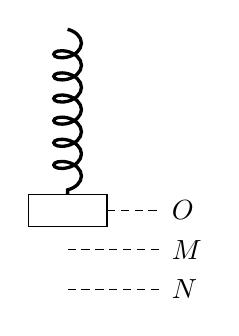
\begin{tikzpicture}
        \wall{(-1,0)}{(1,.2)};
        \draw [very thick,decoration={aspect=.6,segment length=8,amplitude=5,coil},decorate] (0,0) -- (0,-2.1);
        \draw (-.5,-2.5) rectangle (.5,-2.1);
        \draw [densely dashed] (.5,-2.3) -- (1.2,-2.3) node [right] {$O$};
        \draw [densely dashed] (0,-2.8) -- (1.2,-2.8) node [right] {$M$};
        \draw [densely dashed] (0,-3.3) -- (1.2,-3.3) node [right] {$N$};
    \end{tikzpicture}\vspace*{\fill}
\end{problem}
\end{paracol}
\solute0
\begin{solution}
    由于重力、弹簧弹力均为保守力，所以其做功与路径无关，只与始末位置有关.
\end{solution}

\begin{problem} % {牛顿第二定律}
    设物体沿固定圆弧形光滑轨道由静止下滑，在下滑过程中
    \begin{tasks}(2)
        \task 加速度方向永远指向圆心
        \task[\true] 受到的轨道作用力的大小不断增加
        \task 受到的外力大小变化，方向永远指向圆心
        \task 受到的外力大小不变
    \end{tasks}
\end{problem}
\begin{solution}
    物体的加速度由指向圆心的向心加速度和沿运动方向的切向加速度合成，A、C错误. 由于物体的速度不断增大，其向心加速度也不断增大，所以轨道对其作用力不断增大，D错误.
\end{solution}

\begin{paracol}{2}
\begin{problem} % {动能定理，牛顿第二定律}
    如图所示，一质量为$m$的小球，由高$H$处沿光滑轨道由静止开始滑入环形轨道.若$H$足够高，则小球在环最低点时环对它的作用力与小球在环最高点时环对他的作用力之差恰为小球重力的
    \begin{tasks}(4)
        \task $2$倍
        \task $4$倍
        \task[\true] $6$倍
        \task $8$倍
    \end{tasks}
    \switchcolumn\vspace*{\fill}\centering
    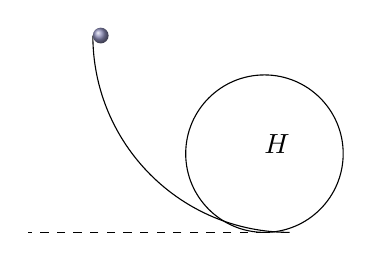
\begin{tikzpicture}
        \draw (0,0) circle (1);
        \draw [dashed] (0,-1) -- (-3,-1);
        \length{(-2.7,-1)}{(-2.7,1.5)}{$H$}{(0,.5)};
        \draw (-2.5,1.5) arc (-180:-90:2.5);
        \shade [ball color=MidnightBlue!50] (-2.4,1.5) circle (.1);
    \end{tikzpicture}\vspace*{\fill}
\end{problem}
\end{paracol}
\solute1
\begin{solution}
    由动能定理$mgH=mv^2/2$得小球在运动到圆轨道底端、顶端时的速率分别为$v_1^2=2gH$，$v_2^2=2g(H-2R)$. 轨道的作用力和小球重力的合力提供向心力，在底端、顶端分别有$N_1-mg=mv_1^2/R$，$N_2+mg=mv_2^2/R$. 所以作用力之差为$N_1-N_2=2mg+m(v_1^2-v_2^2)/R=6mg$.
\end{solution}

\begin{problem} % {动量守恒}
    一质量为$\qty{60}\kg$的人站在一条质量为$\qty{300}\kg$，且正以$\qty2{\m/\s}$的速率向湖岸驶近的小船上，湖水是静止的，其阻力不计.现在人相对于船以水平速率$v$沿船的前进方向向河岸跳去，该人起跳后，船速减为原来一半，$v$应为
    \begin{tasks}(4)
        \task $\qty2{\m/\s}$
        \task $\qty3{\m/\s}$
        \task $\qty5{\m/\s}$
        \task[\true] $\qty6{\m/\s}$
    \end{tasks}
\end{problem}
\solute1
\begin{solution}
    系统水平方向动量守恒，即$(\qty{300}\kg+\qty{60}\kg)\times\qty2{\m/\s}=\qty{60}\kg\times(v+1)+\qty{300}\kg\times \qty1{\m/\s}$. 解得人相对于船的起跳速度$v=\qty6{\m/\s}$.
\end{solution}
\begin{note}
    人相对于船以一水平速率$v$起跳时船速已经变为$\qty1{\m/\s}$. 因为在测得人此时相对于船的速度时，人的脚已经脱离船面，被人蹬完腿后船已经``免费''了. 所以此时人的绝对速度为$(v+1)\unit{\m/\s}$.
\end{note}

\begin{paracol}{2}
\begin{problem} % {高斯定理}
    $A$和$B$为两个均匀带电球体，$A$带电荷$+q$，$B$带电荷$-q$，作一与$A$同心的球面$S$为高斯面，如图所示.则
    \switchcolumn\vspace*{\fill}\centering
    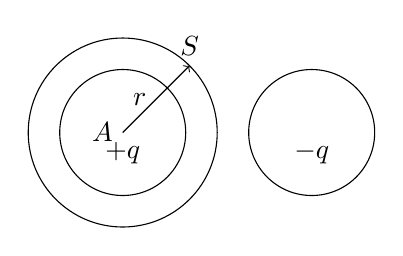
\begin{tikzpicture}
        \draw (0,0) circle (.8) circle (1.2);
        \draw [->] (0,0) node [left] {$A$} node [below] {$+q$} -- (.85,.85) node [midway,left] {$r$} node [above] {$S$};
        \draw (2.4,0) circle (.8) node [below] {$-q$};
    \end{tikzpicture}\vspace*{\fill}
    \switchcolumn
    \begin{tasks}
        \task 通过$S$的通量为零，$S$上各点场强为零.
        \task 通过$S$的通量为$q/\epsilon_0$，$S$上各点场强$E=q/4\pi\epsilon_0r$
        \task 通过$S$的通量为$-q/\epsilon_0$，$S$上各点场强$E=q/4\pi\epsilon_0r$
        \task[\true] 通过$S$的通量为$q/\epsilon_0$，但$S$上各点场强不能直接由高斯定理求出
    \end{tasks}
\end{problem}
\end{paracol}
\begin{solution}
    由高斯定理，通过$S$的电场强度通量为$q/\epsilon_0$. $S$上各点的场强由$+q$和$-q$所激发.
\end{solution}

\begin{problem} % 角量与线量的关系
    一刚体以每分钟$60$转绕$z$轴匀速转动（$\omega$沿$z$轴正向）.某时刻刚体上一点$P$的位置矢量为$r=3\bm i+4\bm j+5\bm k$，单位为``$\qty{e-2}\m$''. 若以``$\qty{e-2}{\m/\s}$''为速度单位，此刻$P$点的速度为
    \begin{tasks}(2)
        \task $\bm v=94.2\bm i+125.6\bm j+157.0\bm k$
        \task[\true] $\bm v=-25.1\bm i+18.8\bm j$
        \task $\bm v=-25.1\bm i-18.8\bm j$
        \task $\bm v=31.4\bm k$
    \end{tasks}
\end{problem}
\solute0
\begin{solution}
    $\bm\omega=60\bm k\unit{r/\min}=2\pi\bm k\unit{\radian/\s}$，$\bm v=\bm\omega\times\bm r=-8\pi\bm i+6\pi\bm j$.
\end{solution}

\begin{problem} % {守恒律}
    一块方板，可以绕通过其一个水平边的光滑固定轴自由转动，最初板自由下落.今有一小团粘土，垂直板面撞击方板，并粘在板上.对粘土和方板系统，如果忽略空气阻力，在碰撞中守恒的量是
    \begin{tasks}(12)
        \task*(2) 动能
        \task*(4)[\true] 绕木板转轴的角动量
        \task*(3) 机械能
        \task*(3) 动量
    \end{tasks}
\end{problem}
\begin{solution}
    二者的碰撞为完全非弹性碰撞，所以动能、机械能不守恒. 二者受转轴水平方向上的作用力，所以动量不守恒. 转轴处的作用力、重力对转轴力矩为零，所以绕转轴的角动量守恒.
\end{solution}

\section{填空题（每空2分，共24分）}

\begin{problem} % {加速度}
    如左下图中所示的三条直线表示同一类型的运动.
    \begin{tasks}[label=\arabic*.](2)
        \task 三条直线表示的是\ans{匀加速直线}运动.
        \task \ans{I}直线所表示的运动的加速度最大.
    \end{tasks}      
\end{problem}

\begin{figure}[htbp]
    \begin{minipage}{.48\textwidth}
        \centering
        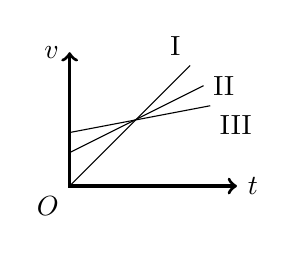
\begin{tikzpicture}[scale=.85]
            \draw [very thick,<->] (2.5,0) node [right] {$t$} -- (0,0) node [below left] {$O$} -- (0,2) node [left] {$v$};
            \draw (0,0) -- (1.8,1.8) node [above left] {I};
            \draw (0,.5) -- (2,1.5) node [right] {II};
            \draw (0,.8) -- (2.1,1.2) node [below right] {III};
        \end{tikzpicture}
    \end{minipage}
    \hfill
    \begin{minipage}{.48\textwidth}
        \centering
        \begin{tikzpicture}[scale=.8]
            \draw [very thick] (-1.2,2.5) -- (1.2,2.5);
            \draw [dashed] (0,2.5) coordinate (o) -- (0,0) coordinate (b);
            \draw (0,0) ellipse (1 and .5);
            \draw (0,2.5) -- (-1,0) coordinate (a) node [midway,left] {$l$};
            \shade[ball color=MidnightBlue!50] (-1,0) circle (.1) node [left] {$m$};
            \pic["$\theta$",draw=DarkRed,ultra thick,angle eccentricity=1.5,angle radius=20]{angle=a--o--b};
        \end{tikzpicture}
    \end{minipage}
\end{figure}

\begin{problem} % {圆周运动，牛顿第二定律}
    如右上图一圆锥摆摆长为$l$，摆锤质量为$m$,在水平面内做匀速圆周运动，摆线与铅直线夹角为$\theta$，则
    \begin{tasks}[label=\arabic*.](2)
        \task 摆线的张力$T=$\ans{$mg/\cos\theta$}.
        \task 摆锤的速率$v=$\ans{$\sin\theta\sqrt{gl/\cos\theta}$}.
    \end{tasks}    
\end{problem}
\begin{solution}\leavevmode
    \begin{enumerate}
        \item 摆锤竖直方向上所受合外力为零，即$T\cos\theta=mg$. 得$T=mg/\cos\theta$.
        \item 摆线张力的水平分量提供向心力，即$T\sin\theta=mv^2/l\sin\theta$. 得$v=\sin\theta\sqrt{gl/\cos\theta}$.
    \end{enumerate}
\end{solution}

\begin{problem} % {相对运动}
    小船以相对于水的速度$\bm v$与水流方向成$\alpha$角运动，若水流速度为$\bm u$，则小船相对于岸的速度的大小为\ans{$\sqrt{v^2+u^2+2uv\cos\alpha}$}，与水流方向的夹角为\ans{$\sin^{-1}(v\sin\alpha/\sqrt{v^2+u^2+2uv\cos\alpha})$}.
\end{problem}
\begin{solution}
    分别由余弦定理、正弦定理即可得出.
\end{solution}

\begin{paracol}{2}
    \begin{problem} % {角动量守恒}
        一根长为$l$的细绳的一段固定于光滑水平面上的$O$点，另一端系一质量为$m$的小球，开始时绳子是松弛的，小球与$O$点的距离为$h$.使小球以某个初速率沿该光滑水平面上一直线运动，该直线垂直于小球初始位置与$O$的连线.当小球与$O$点的距离达到$l$时，绳子绷紧而使小球沿着另一个以$O$点为圆心的圆形轨道运动，则小球作圆周运动时的动能$E_k$与初动能$E_{k_0}$的比值$E_k/E_{k_0}=$\ans{$h^2/l^2$}.
        \switchcolumn\vspace*{\fill}\centering
        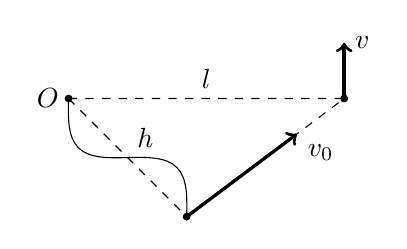
\begin{tikzpicture}
            \draw [dashed] (0,0) -- (1.5,-1.5) node [midway,above right] {$h$} -- (3.5,0) -- cycle node [midway,above] {$l$};
            \draw [very thick,->] (1.5,-1.5) --++ ({1.75*cos(atan(3/4))},{1.75*sin(atan(3/4))}) node [below right] {$v_0$};
            \draw [very thick,->] (3.5,0) --++ (0,{sqrt(2)/2}) node [right] {$v$};
            \draw [rotate around={-45:(0,0)}] (0,0) sin ({.375*sqrt(2)},{-sqrt(2)/4}) cos ({.75*sqrt(2)},0) sin ({1.125*sqrt(2)},{sqrt(2)/4}) cos ({1.5*sqrt(2)},0);
            \fill (0,0) circle (.05) node [left] {$O$};
            \shade [ball color=black] (1.5,-1.5) circle (.05) (3.5,0) circle (.05);
        \end{tikzpicture}\vspace*{\fill}
    \end{problem}
\end{paracol}
\begin{solution}
    由于绳子绷紧后拉力始终指向$O$点，故小球对$O$点角动量守恒，即$mv_0h=mvl$. 由于动能和速度平方成正比，所以动能之比为$E_k/E_{k_0}=v^2/v_0^2=h^2/l^2$.
\end{solution}

\begin{paracol}{2}
\begin{problem} % {转动定律，圆周运动}
    如图所示，一质量为$m$、半径为$R$的薄圆盘，可绕通过其一直径的光滑固定轴$AA'$转动，转动惯量$I=mR^2/4$.该圆盘从静止开始在恒力矩$M$作用下转动，$t$秒后位于圆盘边缘上与轴$AA'$的垂直距离为$R$的$B$点的切向加速度$a_\tau=$\ans{$4M/mR$}，法向加速度$a_n=$\ans{$16M^2t^2/m^2R^3$}.
    \switchcolumn\vspace*{\fill}\centering
    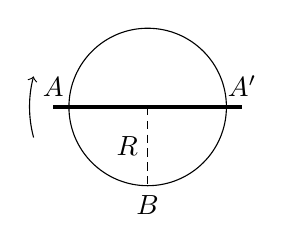
\begin{tikzpicture}
        \draw (0,0) circle (1);
        \draw [very thick] (-1.2,0) node [above] {$A$} -- (1.2,0) node [above] {$A'$};
        \draw [densely dashed] (0,0) -- (0,-1) node [midway,left] {$R$} node [below] {$B$};
        \draw [->] ({-1.5*cos(15)},{-1.5*sin(15)}) arc (195:165:1.5);
    \end{tikzpicture}\vspace*{\fill}
\end{problem}
\end{paracol}
\solute0
\begin{solution}
    圆盘的角加速度$\beta=M/I=4M/mR^2$. 则$B$点切向加速度为$a_\tau=\beta R=4M/mR$. $t$秒后圆盘的角速度$\omega=\beta t=4Mt/mR^2$，$B$点的法向加速度为$a_n=\omega^2R=16M^2t^2/m^2R^3$.
\end{solution}

\begin{paracol}{2}
\begin{problem} % {高斯定理，场强计算}
    一均匀带电直导线长为$d$，电荷线密度为$+\lambda$.过导线中点$O$作一半径为$R$（$R>d/2$）的球面$S$，$P$为带电直导线的延长线与球面$S$的交点.则通过该球面的电场强度通量$\Phi_e=$\ans{$\lambda d/\epsilon_0$}，带电直线的延长线与球面交点$P$处的电场强度的大小为\ans{$\lambda d/4\pi\epsilon_0(R^2-d^2/4)$}，方向\ans{沿矢径$\vv{OP}$}.
    \switchcolumn\vspace*{\fill}\centering
    \begin{tikzpicture}[scale=.6]
        \draw (0,0) circle (2);
        \draw [->] (-2,0) node [left] {$P$} -- (0,0) node [above] {$O$} -- (1,{sqrt(3)}) node [above right] {$R$};
        \filldraw (-2,0) circle (.05);
        \filldraw [pattern=north east lines] (-.8,-.1) -- (-.8,.1) -- (.8,.1) -- (.8,-.1)--cycle;
        \length{(-.8,-.5)}{(.8,-.5)}{$d$}{(.5,0)};
    \end{tikzpicture}\vspace*{\fill}
\end{problem}
\end{paracol}
\begin{solution}\leavevmode
    \begin{itemize}
        \item 由高斯定理得$\Phi_e=\lambda d/\epsilon_0$.
        \item 带电线上$x\sim x+\d x$的一段线元在$P$处产生的场强大小为$\d E=\d q/[4\pi\epsilon_0(R-x)^2]$.
        \item 对其积分得$E=\displaystyle\int_{-d/2}^{d/2}\frac{1}{4\pi\epsilon_0}\frac{\lambda\d x}{(R-x)^2}=\frac{\lambda d}{4\pi\epsilon_0(R^2-d^2/4)}$，方向水平向左（沿矢径$\vv{OP}$）.
    \end{itemize}
\end{solution}
\solute*{为节约资源，本试题计算题部分不提供演算区域，请自备稿纸，或在下页边缘书写.}

\section{计算题（共46分）}

\begin{problem} % {转动定律}
    一转动惯量为$I$的圆盘绕一端固定轴转动，起初角速度为$\omega_0$.设它所受阻力矩与转动叫速度成正比，即$M=-k\omega$（$k>0$）.求圆盘的角速度从$\omega_0$变为$\omega_0/2$时所需时间.
\end{problem}
\begin{solution}
    由转动定律得$\beta=\d\omega/\d t=M/I=-k\omega/I$. 分离变量积分并代入初始条件得$\omega(t)=\omega_0\e^{-kt/I}$. 当$\omega=\omega_0/2$时，$t=I\ln 2/k$.
\end{solution}

\begin{problem} % {速度与速率}
    一人自原点出发，$\qty{25}\s$内向东走$\qty{30}\m$，又$\qty{10}\s$内向南走$\qty{10}\m$，再$\qty{15}\s$内向正西北走$\qty{18}\m$.求在这$\qty{50}\s$内
    \begin{tasks}[label=\arabic*.](2)
        \task 平均速度的大小和方向.
        \task 平均速率的大小.
    \end{tasks}
\end{problem}
\begin{solution}\leavevmode
    \begin{enumerate}
        \item
        \begin{itemize}
            \item $\overline{\bm v}=\Delta\bm x/\Delta t=(30\bm i-10\bm j-18\bm i/\sqrt{2}+18\bm j/\sqrt{2})/50=(0.345\bm i+0.0546\bm j)\unit{\m/\s}$.
            \item 其大小$\abs{\overline{\bm v}}=0.3\qty5{\m/\s}$，方向$\theta=\arctan{0.0546/0.345}=\qty{8.98}\degree$.
        \end{itemize}
        \item $\overline v=\Delta s/\Delta t=(30+10+18)/50=\qty{1.16}{\m/\s}$.
    \end{enumerate}
\end{solution}

\begin{problem} % {牛顿第二定律}
    如图左下所示，质量为$m$的摆球$A$悬挂在车架上.求在下述各种情况下，摆球与竖直方向的夹角$\alpha$和线中的张力$T$.
    \begin{enumerate}
        \item 小车沿水平方向做匀速运动.
        \item 小车沿水平方向做加速度为$\bm a$的运动.
    \end{enumerate}
\end{problem}
\begin{solution}\leavevmode
    \begin{enumerate}
        \item 此时线处于竖直方向，此方向上摆球的受力平衡，即$\alpha=0$，$T=mg$.
        \item 引入惯性力$-m\bm a$，摆球分别在水平和竖直方向上受力平衡，即$T\sin\alpha=ma$，$T\cos\alpha=mg$. 得$\alpha=\arctan{a/g}$，$T=m\sqrt{a^2+g^2}$.
    \end{enumerate}
\end{solution}

\begin{figure}[htbp]
    \begin{minipage}{.48\textwidth}
        \centering
        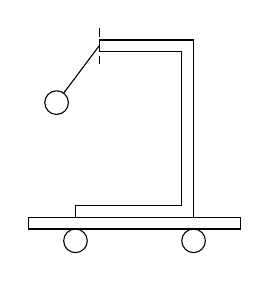
\begin{tikzpicture}[scale=.75]
            \wall{(-2,0)}{(2,-.3)};
            \draw (-1,.2) circle (.2);
            \draw (1,.2) circle (.2);
            \draw (-1.8,.4) rectangle (1.8,.6);
            \draw (-1,.6) -- (1,.6) -- (1,3.6) -- (-.6,3.6) -- (-.6,3.4) -- (.8,3.4) -- (.8,.8) -- (-1,.8) -- cycle;
            \draw [densely dashed] (-.6,3.8) -- (-.6,3.2);
            \draw (-.6,3.5) --++ (-.6,-.8) ++ (-.12,-.16) circle (.2);
        \end{tikzpicture}
    \end{minipage}
    \hfill
    \begin{minipage}{.48\textwidth}
        \centering
        \begin{tikzpicture}
            \length{(-.3,0)}{(-.3,2)}{$h$}{(0,.75)};
            \draw (0,0) -- (2.5,0) arc (90:-90:.2) -- (0,-.4) arc (270:90:.2)--cycle;
            \draw [->] (.8,-.12) -- (1.7,-.12);
            \draw [<-] (.8,-.52) -- (1.7,-.52);
            \draw (0,-.2) circle (.2);
            \draw (2.5,-.2) circle (.2);
            \filldraw [pattern=north east lines] (0,0) -- (2.5,0) -- (2.4,.1) -- (.1,.1)--cycle;
            \draw (-.2,2.5) -- (0,2) -- (1.5,2) -- (1.7,2.5);
        \end{tikzpicture}
    \end{minipage}
\end{figure}

\begin{problem} % {冲量与动量定理}
    如右上图所示，传送带以$\qty3{\m/\s}$的速率水平向右运动，砂子从高$h=\qty{0.8}\m$处落到传送带上，即随之一起运动. 求传送带给砂子的作用力的方向（重力加速度$g$取$\qty{10}{\m/\s^2}$）.
\end{problem}
\begin{solution}\leavevmode
    \begin{itemize}
        \item 质量为$\d m$的砂子在接触传送带前的速度为$v=\sqrt{2gh}$，方向竖直向下.
        \item 接触传送带前后瞬间，其动量分别为$\bm p=-\sqrt{2gh}\d m\bm j=-\qty4{\m/\s}\bm j$，$\bm p'=\qty3{\m/\s}\cdot\d m\bm i$.
        \item 砂子的动量变化为$\Delta\bm p=\bm p'-\bm p=\qty3{\m/\s}\d m\bm i+\qty4{\m/\s}\d m\bm j$.
        \item 由动量定理，传送带给砂子的作用力方向与砂子的动量变化方向相同（不考虑重力）. 
        \item 传送带给砂子的作用力方向与水平面的夹角为$\theta=\arctan4/3=53^{\circ}$，方向斜向上.
    \end{itemize}
\end{solution}

\begin{problem} % {动量守恒}
    一电子和一个静止着的氢原子发生对心完全弹性碰撞.已知氢原子质量为电子质量的$1840$倍，求碰撞过程中传给氢原子的能量与电子原来能量的比值.
\end{problem}
\begin{solution}
    设电子质量为$m$，氢原子质量为$1840m$，电子速率为$v_0$.碰撞过程中氢原子和电子组成的系统动量守恒
    \[mv_0=mv_1+1840mv_2\]
    由于碰撞为完全弹性碰撞，所以碰撞过程中能量守恒
    \[\frac12mv_0^2=\frac12mv_1^2+\frac12\cdot 1840 mv_2^2\]
    联立以上两式得$\Delta E_k/E_{k_0}=1840v_2^2/v_0^2=\num{2.17e-3}$.
\end{solution}

\begin{paracol}{2}
\begin{problem} % {场强计算}
    真空中两条平行的``无限长''均匀带电直线相距为$a$，其电荷线密度分别为$-\lambda$和$+\lambda$. 试求
    \begin{enumerate}
        \item 在两直线构成的平面上，两线间任一点的电场强度（选$Ox$轴如图所示，两线的中点为原点）.
        \item 两带电直线上单位长度之间的相互吸引力.
    \end{enumerate}
\end{problem}
\switchcolumn\centering
\vfill
\begin{tikzpicture}
    \draw [->] (-2,0) -- (2,0) node [midway,below] {$O$} node [below] {$x$};
    \shade [ball color=black] (0,0) circle (.05);
    \draw (-1.2,-1) -- (-1.2,1);
    \draw [dashed] (-1.2,-1.5) -- (-1.2,1.5) node [above] {$-\lambda$};
    \draw (1.2,-1) -- (1.2,1);
    \draw [dashed] (1.2,-1.5) -- (1.2,1.5) node [above] {$+\lambda$};
    \length{(-1.2,.9)}{(1.2,.9)}{$a$}{(.5,0)};
\end{tikzpicture}
\vfill
\end{paracol}
\begin{solution}\leavevmode
    \begin{enumerate}
        \item $x$处的场强由$-\lambda$和$+\lambda$的带电直线所产生. 根据无限长均匀带电直线周围的场强分布
        \[E=-\frac{\lambda}{2\pi\epsilon_0(x+a/2)}+\frac{\lambda}{2\pi\epsilon_0(a/2-x)}=\frac{2a\lambda}{\pi\epsilon_0(a^2-4x^2)}\]
        \item $\Delta F=\lambda E=\lambda^2/2\pi\epsilon_0a$.
    \end{enumerate}
\end{solution}

\begin{multicols}{2}
\begin{problem} % {场强计算}
    一半径为$R$的带电球体，其电荷体密度分别为（其中$q$为一正的常量）
    \[\begin{cases}
        \rho=\dfrac{qr}{\pi R^4}&(r\leq R)\\
        \rho=0&(r>R)
    \end{cases}\]
    \begin{enumerate}
        \item 求带电球体的总电荷.
        \item 求球内、外各点的电场强度.
    \end{enumerate}
\end{problem}
\begin{solution}\leavevmode
    \begin{enumerate}
        \item $Q=\displaystyle\iiint{\rho\d V}=\int_0^R{\frac{qr}{\pi R^4}4\pi r^2\d r}=q$.
        \item 取$r<R$和$r\ge R$的高斯面，由高斯定理
        \[E=\begin{cases}
            \displaystyle\frac{\int_0^r{\rho\cdot4\pi r^2\d r}}{4\pi\epsilon_0r^2}=\frac{1}{4\pi\epsilon_0}\frac{qr^2}{R^4} & r<R\\
            \displaystyle\frac{1}{4\pi\epsilon_0}\frac{q}{r^2} & r\geq R
        \end{cases}\]
    \end{enumerate}
\end{solution}
\end{multicols}